% --------------------------------------------------------------------------------

\begin{exercise}

Sei $\Omega$ eine beschränkte Teilmenge von $\R^n$ mit $C^{\infty}$-Rand und $\1_\Omega$ ihre Indikatorfunktion.
Zeigen Sie

\begin{align*}
  \abraces{\Delta \1_\Omega, \varphi}
  =
  \Int[\partial \Omega]{\pderivative[][\varphi]{\nu}}{s},
\end{align*}

wobei $\nu$ der äußere Normaleneinheitsvektor auf $\partial \Omega$ ist.

\end{exercise}

% --------------------------------------------------------------------------------

\begin{solution}

Klarerweise ist $\1_\Omega \in L^1_{\mathrm{loc}}$.
Somit ist der Ausdruck auf der linken Seite, als Linearkkombination von Ableitungen von dieser Distribution, wohldefiniert.
Der Laplace-Operator $\Delta$ ist formal selbstadjungiert und $\Delta = \Div(\nabla)$.
Wenn wir $\Omega$ als offen annehmen, können wir den Satz von Gauß anwenden
(ansonsten müssen wir uns noch was einfallen lassen):
\begin{figure}[h!]
  \centering
  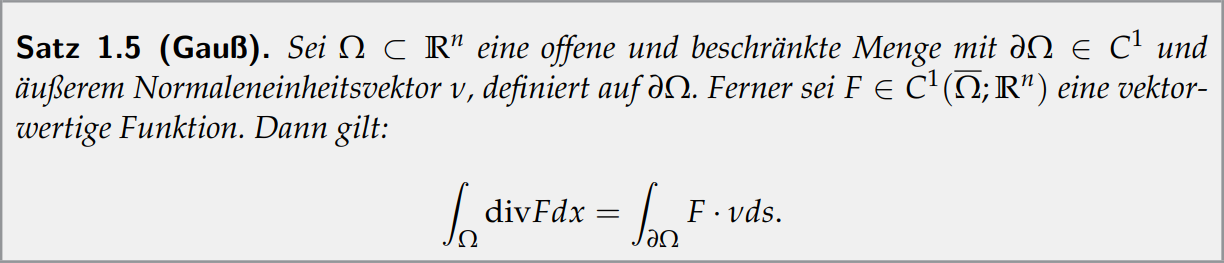
\includegraphics[width = 0.75 \textwidth]{Satz 1-5 (Gauss).png}
\end{figure}

\begin{multline*}
  \implies
  \langle \Delta \1_\Omega, \varphi \rangle
  =
  \langle  \1_\Omega, \Delta \varphi \rangle
  =
  \Int[\R^n]{\1_\Omega \Delta \varphi}{x}
  =
  \Int[\Omega]{\Delta \varphi}{x}
  =
  \Int[\Omega]{\Div(\nabla \varphi)}{x} \\
  \stackrel{\text{Gauß}}{=}
  \Int[\partial \Omega]{\nabla \varphi \cdot \nu}{s}
  =
  \Int[\partial \Omega]{\frac{\partial \varphi}{\partial \nu}}{s}
\end{multline*}

\end{solution}

% --------------------------------------------------------------------------------
